\section{Introduction}

\subsection{Motivation}

\begin{frame}{Motivation}
    \begin{itemize}
        \item Data often come with different sizes and shapes
        \item All machine learning models require some properties on data
    \end{itemize}
\end{frame}

\begin{frame}{Different sizes and shapes}
    \begin{columns}
    \begin{column}{0.5\textwidth}
       \begin{itemize}
        \item Different representations
        \item Missing values / Noisy data
    \end{itemize}
    \end{column}
    \begin{column}{0.5\textwidth}
        \begin{center}
        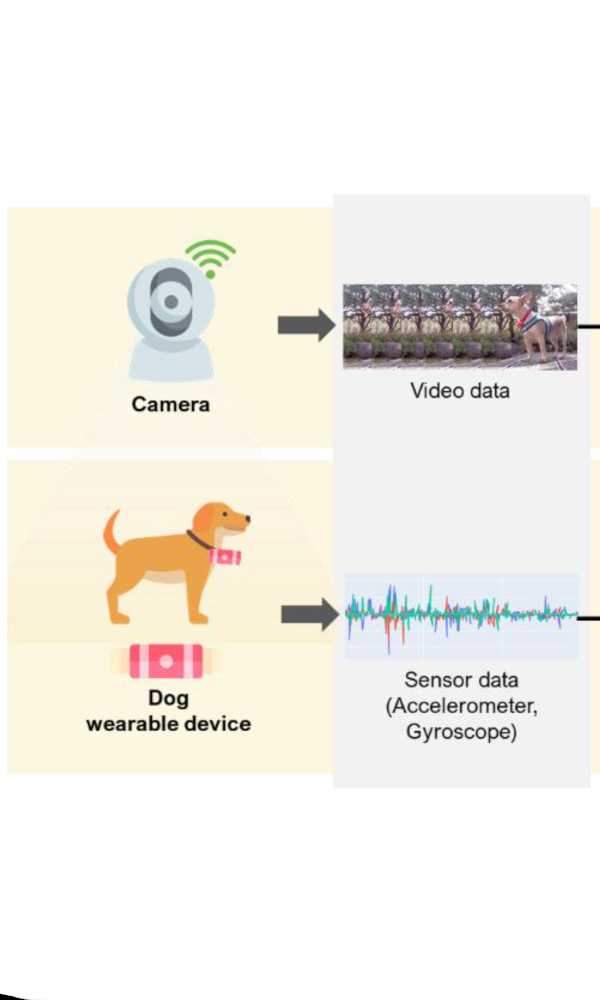
\includegraphics[width=0.7\textwidth]{assets/data_sizes_shapes.png}
        \end{center}
    \end{column}
    \end{columns}
    
\end{frame}


\begin{frame}{Assumption on Data}
    \begin{itemize}
        \item A dataset come from a specific distribution
    \end{itemize}
    
    \begin{table}[h]
        \centering
        \begin{tabular}{c|c}
            Model & Assumption \\
            \hline
            Linear Regression & Linear relationship  \\
            Support vector machines & Linear Separable \\
            Gaussian Mixture Model & Mixture of Gaussians \\
            Semi-supervised & Continuity, Cluster, Manifold \\
            ... & ... \\
        \end{tabular}
    \end{table}
\end{frame}

\subsection{Outline}

\begin{frame}{Outline}

\begin{outline}
\1 Data Pre-processing
    \2 Structured Data
        \3 Data Cleaning
        \3 Data Integration
        \3 Data Reduction
        \3 Data Discretization and Transformation
    \2 Unstructured data
        \3 Image
        \3 Audio
\1 Data Post-processing
    \2 Model evaluation
    \2 Comparing Models
\end{outline}
    
\end{frame}